\documentclass[compress]{beamer}

\usepackage{graphicx,epstopdf,subfigure,booktabs,natbib}

\usepackage{tikz}
\usetikzlibrary{shapes,arrows,calc,through,backgrounds,shapes.symbols,positioning}

%\usetheme[compress,subsection=F]{Singapore}
\useoutertheme[subsection=false]{miniframes}
\useinnertheme{default}
\usecolortheme{seagull}


\bibliographystyle{plainnat}
\bibpunct{[}{]}{;}{a}{}{,}

% for themes, etc.

% these will be used later in the title page
\title[TITLE]{TITLE}
\subtitle{SUBTITLE}
\author[Bracken]{Cameron Bracken\footnote{Humboldt State University}}
\date{DATE}


\begin{document}

\begin{frame}
\titlepage
\end{frame}

\section{Ways to be cool}

\subsection{Cool ways to say hello}
\begin{frame}{Cool ways to say hello}
	\begin{itemize}
		\item yo dawg
		\item what up 
		\item hows it go
		\item *jerk chin up slightly*
	\end{itemize}
\end{frame}

\subsection{Cool hair styles}
\begin{frame}{Cool hair styles}
	\begin{itemize}
		\item Afros
		\item CRAZY bed head
		\item Poof in the front 
		\item Mohawks
	\end{itemize}
	If you follow these things you will be cool.
\end{frame}


\subsection{Example of a PGF flow chart}
\begin{frame}{Example of a PGF flow chart}

	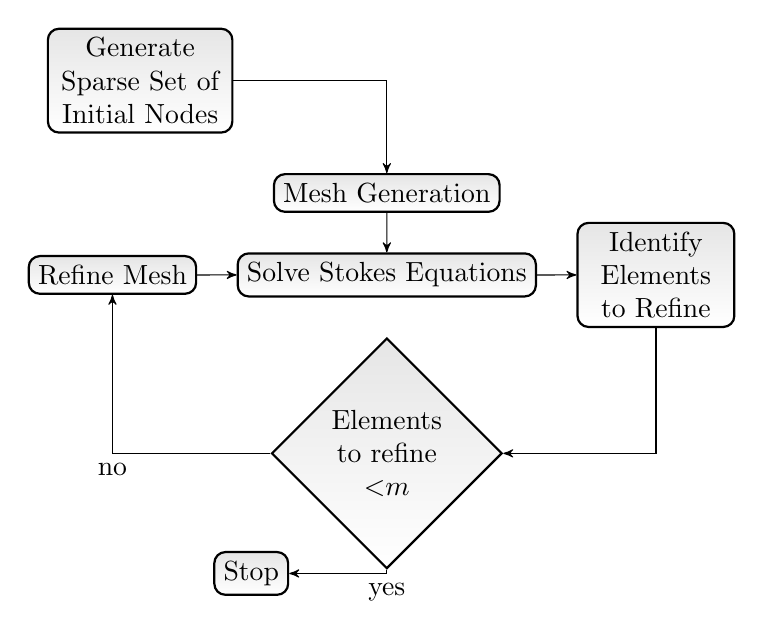
\begin{tikzpicture}[node distance=5mm and 5mm,scale=.8,
	decision/.style={diamond, draw=black, thick, top color=gray!20, bottom color=white,
	text width=5em, text badly centered, 
	inner sep=.5pt}, 
	block/.style ={rectangle, draw=black, thick, top color=gray!20, bottom color=white,
	rounded corners,
	},] 

	\node (init)[block, text badly centered,text width=6em] {Generate Sparse Set of Initial Nodes};
	\pause 
	\node(gen) [block,below right=of init] {Mesh Generation};
	\draw[-stealth'] (init) -| (gen); 
	\pause

	\node(solve)[block,below=of gen] {Solve Stokes Equations};   
	\draw[-stealth'] (gen) -- (solve);
	\pause

	\node(elements) [block,right=of solve,text width=5em,text badly centered] {Identify Elements to Refine}; 
	\draw[-stealth'] (solve) -- (elements);
	\pause

	\node(decide)[decision,below=of solve] {Elements to refine $<$$m$};  
	\draw[-stealth'] (elements) |- (decide); 
	\pause

	\node(update) [block,left=of solve] {Refine Mesh}; 
	\draw[-stealth'] (decide) -| node [below] {no} (update);
	\pause

	\draw[-stealth'] (update) -- (solve); 
	\pause
 
	\node (stop)[block,below left=of decide] {Stop}; 
	\draw[-stealth'] (decide) |- node [below] {yes} (stop); 

	\end{tikzpicture}\\ 
	\only<1-7>{~}
	\only<8>{How is this efficient?}
\end{frame}

\end{document}  